\noindent Typické softvérové aplikácie na spracovanie jazyka sa
skladajú z~niekoľkých zložiek, ktoré odrážajú rôzne aspekty
jazyka a~úlohu, ktorú plnia. Obrázok~\ref{fig:textprocessingarch_sk}
zobrazuje veľmi zjednodušenú architektúru, ktorú možno nájsť
v~systéme na spracovanie textu. Prvé tri moduly sa zaoberajú
štruktúrou a~významom textového vstupu:

\begin{figure*}[ht]
  \colorrule{grey3}{\textwidth}{1.5pt}
  \center
  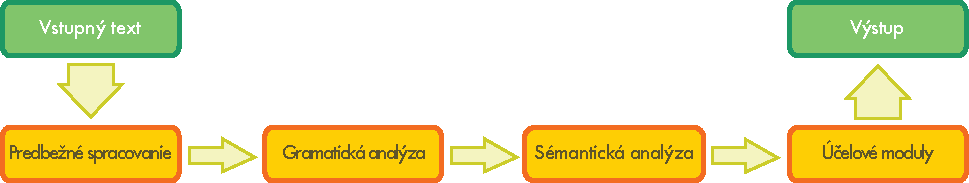
\includegraphics[width=\textwidth]{../_media/slovak/text_processing_app_architecture}
  \caption{Typická architektúra aplikácie na spracovanie textu}
  \label{fig:textprocessingarch_sk}
  \colorrule{grey3}{\textwidth}{1.5pt}
\end{figure*}

\begin{itemize}
\item Predbežné spracovanie: vyčistenie dát, odstránenie formátovania, detekcia vstupného jazyka, detekcia chýbajúcej diakritiky atď.
\item Gramatická analýza: hľadanie slovesa a~jeho prislúchajúceho predmetu alebo zvratného zámena atď.; zistenie vetnej štruktúry.
\item Sémantická analýza: odstránenie viacznačnosti (Ktorý význam slova \emph{mier} je správny v~danom kontexte?), vyriešenie anafory a~odkazujúcich výrazov ako \emph{on}, \emph{to auto} atď.; prezentácia významu vety v~strojovo čitateľnej forme.	
\end{itemize}

Moduly na špecifické úlohy potom vykonávajú rôzne operácie, ako je
automatická sumarizácia vstupného textu, databázové hľadania
a~mnoho ďalších. Ďalej ukážeme základné aplikačné oblasti
a~zdôrazníme ich základné moduly. Opäť pripomíname,
že architektúry aplikácií sú veľmi zjednodušené a~idealizované
pre vyjadrenie komplexnosti aplikácií jazykových technológií
všeobecne zrozumiteľným spôsobom.

Po predstavení základných aplikačných oblastí poskytneme stručný
prehľad situácie jazykových technológií v~oblasti výskumu a~vzdelávania, pričom na záver uvedieme prehľad minulých
a~prebiehajúcich výskumných programov. Na konci tejto časti budeme
prezentovať odborný odhad situácie oblasti základných nástrojov
a~zdrojov jazykových technológií z~viacerých hľadísk, napríklad z hľadiska dostupnosti, zrelosti alebo kvality. Táto tabuľka poskytne
prehľad situácie jazykových technológií pre slovenčinu.


